\section{Tekis o‘zgaruvchan harakatni grafik ravishda tasvirlash}

\begin{enumerate}

\item Rasmda 5 ta jism tezliklarining vaqtga bog‘lanish grafiklari keltirilgan. 
Qaysi jismlar tekis harakat qiladi?

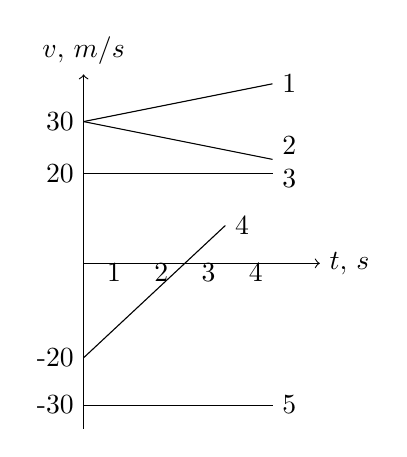
\begin{tikzpicture}[scale=0.6]

% o'qlar
\draw[->] (0,-3.5) -- (0,4) node[above] {$v,\,m/s$};
\draw[->] (0,0) -- (5,0) node[right] {$t,\,s$};

% belgilar
\node[left] at (0,3) {30};
\node[left] at (0,1.9) {20};
\node[left] at (0,-2) {-20};
\node[left] at (0,-3) {-30};

\node[left] at (1,-0.2) {1};
\node[left] at (2,-0.2) {2};
\node[left] at (3,-0.2) {3};
\node[left] at (4,-0.2) {4};
% chiziqlar
\draw (0,3) -- (4,3.8);      % 1
\draw (0,3) -- (4,2.2);      % 2
\draw (0,1.9) -- (4,1.9);        % 3
\draw (0,-2) -- (3,0.8);     % 4
\draw (0,-3) -- (4,-3);      % 5

% raqamlar
\node[right] at (4,3.8) {1};
\node[right] at (4,2.5) {2};
\node[right] at (4,1.8) {3};
\node[right] at (3,0.8) {4};
\node[right] at (4,-3) {5};

\end{tikzpicture}


\begin{enumerate}[label=\Alph*)]
\item 1,4
\item 2
\item 1,2,4
\item 3,5
\end{enumerate}


\item Rasmda jism tezlanishining vaqtga bog‘lanishi berilgan. 
Vaqtning qaysi oralig‘ida jism tekis tezlanuvchan harakat qilgan?

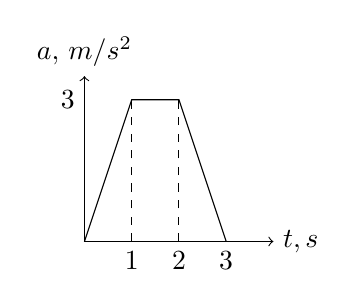
\begin{tikzpicture}[scale=0.6]

\draw[->] (0,0) -- (4,0) node[right] {$t,s$};
\draw[->] (0,0) -- (0,3.5) node[above] {$a,\,m/s^2$};

\node[left] at (0,3) {3};

\draw (0,0) -- (1,3) -- (2,3) -- (3,0);

\draw[dashed] (1,0) -- (1,3);
\draw[dashed] (2,0) -- (2,3);

\node[below] at (1,0) {1};
\node[below] at (2,0) {2};
\node[below] at (3,0) {3};

\end{tikzpicture}


\begin{enumerate}[label=\Alph*)]
\item 2–3
\item 1–2
\item 0–1
\item 0–1, 2–3
\end{enumerate}


\item Quyidagi grafikdagi $\alpha$ burchak tangensi qanday fizik ma’noga ega?

\begin{tikzpicture}[scale=0.6]

\draw[->] (0,0) -- (4,0) node[right] {$t$};
\draw[->] (0,0) -- (0,3) node[above] {$v$};

\draw (0,0) -- (3.2,2);

\draw (0.9,0) arc (0:32:0.9);
\node at (1.3,0.45) {$\alpha$};

\node at (-0.1,-0.1) {$0$};

\end{tikzpicture}

\begin{enumerate}[label=\Alph*)]
\item tezlanish o‘zgarishi
\item tezlanish
\item tezlik o‘zgarishi
\item tezlik
\end{enumerate}


\item Keltirilgan grafikdan foydalanib, jismning harakat tezlanishini toping (m/s$^2$).

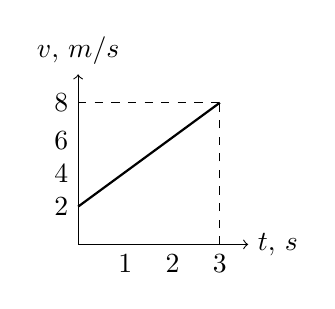
\begin{tikzpicture}[scale=0.6]

\draw[->] (0,0) -- (3.6,0) node[right] {$t,\,s$};
\draw[->] (0,0) -- (0,3.6) node[above] {$v,\,m/s$};

\draw[dashed] (0,3) -- (3,3);
\draw[dashed] (3,0) -- (3,3);

\node[left] at (0,3) {8};
\node[left] at (0,2.2) {6};
\node[left] at (0,1.5) {4};
\node[left] at (0,0.8) {2};

\node[below] at (1,0) {1};
\node[below] at (2,0) {2};
\node[below] at (3,0) {3};

\draw[thick] (0,0.8) -- (3,3);

\end{tikzpicture}

\begin{enumerate}[label=\Alph*)]
\item 3
\item 6
\item 2
\item 4
\end{enumerate}


\item Jism tezligining vaqtga bog‘lanish grafigi rasmda ko‘rsatilgan. 
1-, 2- va 3- nuqtalarga mos keluvchi tezlanishlarni taqqoslang.

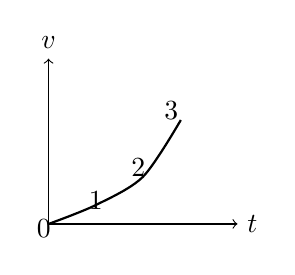
\begin{tikzpicture}[scale=0.6]

\draw[->] (0,0) -- (4,0) node[right] {$t$};
\draw[->] (0,0) -- (0,3.5) node[above] {$v$};

\draw[thick] plot[smooth] coordinates {(0,0)(1,0.4)(2,1)(2.8,2.2)};

\node at (1,0.5) {1};
\node at (1.9,1.2) {2};
\node at (2.6,2.4) {3};

\node at (-0.1,-0.1) {$0$};

\end{tikzpicture}

\begin{enumerate}[label=\Alph*)]
\item $a_1<a_2<a_3$
\item $a_2>a_1>a_3$
\item $a_1>a_2>a_3$
\item $a_2<a_1<a_3$
\end{enumerate}




\item Rasmda to‘g‘ri chiziqli harakat qilayotgan jismning tezlik grafigi keltirilgan. Bu harakatning tezlik tenglamasi qanday bo‘ladi?

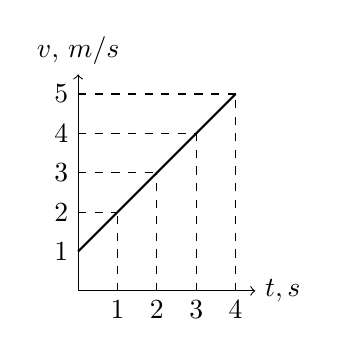
\begin{tikzpicture}[scale=0.5]

\draw[->] (0,0) -- (4.5,0) node[right] {$t,s$};
\draw[->] (0,0) -- (0,5.5) node[above] {$v,\,m/s$};

\draw[dashed] (0,5) -- (4,5);
\draw[dashed] (0,4) -- (3,4);
\draw[dashed] (0,3) -- (2,3);
\draw[dashed] (1,0) -- (1,2);
\draw[dashed] (0,2) -- (1,2);
\draw[dashed] (3,0) -- (3,4);
\draw[dashed] (4,0) -- (4,5);

\node[left] at (0,1) {1};
\node[left] at (0,2) {2};
\node[left] at (0,3) {3};
\node[left] at (0,4) {4};
\node[left] at (0,5) {5};

\foreach \x in {1,2,3,4}
\node[below] at (\x,0) {\x};

\draw[thick] (0,1) -- (4,5);

\draw[dashed] (2,0) -- (2,3);
\draw[dashed] (0,3) -- (2,3);

\end{tikzpicture}

\begin{enumerate}[label=\Alph*)]
\item $v = 1 + 2t$
\item $v = 1 + t$
\item $v = 2 + 2t$
\item $v = 2 + t$
\end{enumerate}


\item Jism rasmdagi kabi tekis o‘zgaruvchan harakatlanmoqda. 
Tezlanish yo‘nalishi o‘zgarmagan. 
Jismning 8 s da o‘tgan yo‘li (m) va ko‘chishini aniqlang (m).

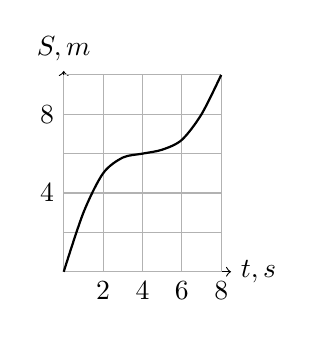
\begin{tikzpicture}[scale=0.25]

\draw[->] (0,0) -- (8.5,0) node[right] {$t,s$};
\draw[->] (0,0) -- (0,10.2) node[above] {$S,m$};

\draw[step=2cm,gray!60] (0,0) grid (8,10);

\node[left] at (0,4) {4};
\node[left] at (0,8) {8};

\node[below] at (2,0) {2};
\node[below] at (4,0) {4};
\node[below] at (6,0) {6};
\node[below] at (8,0) {8};

\draw[thick,smooth]
plot coordinates {(0,0)(1,3)(2,5)(3,5.8)(4,6)(5,6.2)(6,6.7)(7,8)(8,10)};

\end{tikzpicture}

\begin{enumerate}[label=\Alph*)]
\item 10; 10
\item 6; 10
\item 8; 4
\item 10; 1
\end{enumerate}


\item Quyida turli jismlarning tezlik grafiklari keltirilgan. 
Ularning qaysi biri shaharlararo yo‘ldan ketayotib, biror sabab bilan 
yo‘l chetiga chiqib to‘xtagan avtobus harakatini tavsiflashi mumkin?

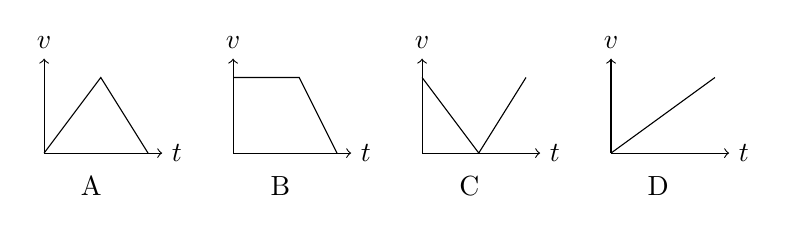
\begin{tikzpicture}[scale=0.6]

% A
\begin{scope}
\draw[->] (0,0)--(2.5,0) node[right] {$t$};
\draw[->] (0,0)--(0,2) node[above] {$v$};
\draw (0,0)--(1.2,1.6)--(2.2,0);
\node at (1,-0.7) {A};
\end{scope}

% B
\begin{scope}[xshift=4cm]
\draw[->] (0,0)--(2.5,0) node[right] {$t$};
\draw[->] (0,0)--(0,2) node[above] {$v$};
\draw (0,1.6)--(1.4,1.6)--(2.2,0);
\node at (1,-0.7) {B};
\end{scope}

% C
\begin{scope}[xshift=8cm]
\draw[->] (0,0)--(2.5,0) node[right] {$t$};
\draw[->] (0,0)--(0,2) node[above] {$v$};
\draw (0,1.6)--(1.2,0)--(2.2,1.6);
\node at (1,-0.7) {C};
\end{scope}

% D
\begin{scope}[xshift=12cm]
\draw[->] (0,0)--(2.5,0) node[right] {$t$};
\draw[->] (0,0)--(0,2) node[above] {$v$};
\draw (0,0)--(2.2,1.6);
\node at (1,-0.7) {D};
\end{scope}


\end{tikzpicture}



\item Rasmda ko‘rsatilgan grafikdan foydalangan holda birinchi va ikkinchi jismlar 4 s davomidagi ko‘chishlarining farqi topilsin(m).

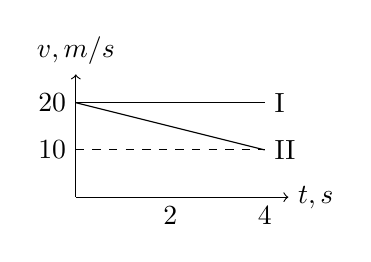
\begin{tikzpicture}[scale=0.6]
\draw[->] (0,0) -- (4.5,0) node[right] {$t,s$};
\draw[->] (0,0) -- (0,2.6) node[above] {$v,m/s$};

\node[left] at (0,2) {20};
\node[left] at (0,1) {10};

\node[below] at (2,0) {2};
\node[below] at (4,0) {4};

\draw (0,2) -- (4,2);
\draw (0,2) -- (4,1);

\draw[dashed] (0,1) -- (4,1);

\node[right] at (4,2) {I};
\node[right] at (4,1) {II};

\end{tikzpicture}

\begin{enumerate}[label=\Alph*)]
\item 20
\item 30
\item 40
\item 60
\end{enumerate}


\item Rasmda jism tezligining vaqtga bog‘lanish grafigi keltirilgan. 
Jismning $(3\,\text{s},\,8\,\text{s})$ vaqt oralig‘ida bosib o‘tgan yo‘li (m) topilsin.

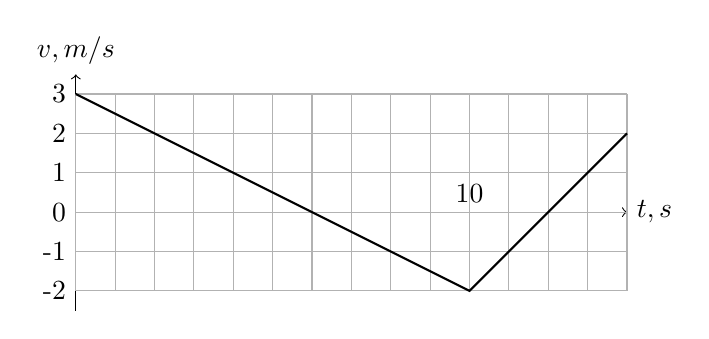
\begin{tikzpicture}[scale=0.5]

\draw[->] (0,0) -- (14,0) node[right]{$t,s$};
\draw[->] (0,-2.5) -- (0,3.5) node[above] {$v,m/s$};

\draw[step=1cm,gray!60] (0,-2) grid (14,3);

\draw[thick] (0,3) -- (10,-2) -- (14,2);

\node[above] at (10,0) {10};
\node[left] at (0,0) {0};
\node[left] at (0,1) {1};
\node[left] at (0,2) {2};
\node[left] at (0,3) {3};
\node[left] at (0,-1) {-1};
\node[left] at (0,-2) {-2};

\end{tikzpicture}

\begin{enumerate}[label=\Alph*)]
\item 1,3
\item 1,75
\item 1,45
\item 3,25

\end{enumerate}


\item Quyida jism tezligining vaqtga bog‘langan grafigi keltirilgan bo‘lib, 
uning $0-8$ s oraliqdagi o‘rtacha tezligi 17 m/s ga teng ekanligi ma’lum. 
Bundan foydalanib, jismning $0-4$ s oraliqdagi o‘rtacha tezligini toping (m/s).

\begin{tikzpicture}[scale=0.6]

\draw[->] (0,0) -- (4,0) node[right] {$t,s$};
\draw[->] (0,0) -- (0,4) node[above] {$v,m/s$};

\node[left] at (0,3) {$v$};
\node[left] at (0,1.5) {8};

\node[below] at (2,0) {4};
\node[below] at (4,0) {8};

\draw (0,1.5) -- (2,3);
\draw (2,3) -- (4,3);

\draw[dashed] (4,0) -- (4,3);
\draw[dashed] (2,0) -- (2,3);

\end{tikzpicture}

\begin{enumerate}[label=\Alph*)]
\item 13
\item 15
\item 14
\item 12

\end{enumerate}


\item Quyida boshlang‘ich tezligi $10\ \text{m/s}$ bo‘lgan jism tezlanishining 
vaqtga bog‘lanish grafigi tasvirlangan. 
Jism 20 s da 500 m yo‘l yurgan bo‘lsa, $a$ nimaga teng (m/s$^2$)?

\begin{tikzpicture}[scale=0.6]

\draw[->] (0,0) -- (11,0) node[right] {$t,s$};
\draw[->] (0,0) -- (0,3) node[above] {$a,m/s^2$};

\node[left] at (0,2) {$a$};

\node[below] at (5,0) {10};
\node[below] at (10,0) {20};

\draw[very thick] (0,2) -- (5,2);
\draw[very thick] (5,0) -- (10,0);
\draw[dashed] (5,0) -- (5,2);

\end{tikzpicture}

\begin{enumerate}[label=\Alph*)]
\item 1,5
\item 2
\item 2,5
\item 3
\end{enumerate}

\end{enumerate}



\begin{table}[h!]
\centering
\begin{tabular}{|c|c|c|c|c|c|c|c|c|c|}
\hline
1d & 2b & 3b & 4c & 5a & 6b & 7a & 8c & 9a & 10d \\ \hline
11c & 12b &  &  &  &  &  &  &  &  \\ \hline
\end{tabular}
\end{table}